\chapter{Fundamente}


\section{Rețea neurală}
O rețea neurală este un ansamblu interconectat de elemente de procesare simple, \textit{unități} sau \textit{noduri}, a căror funcționalitate este ușor bazată pe neuronul biologic. Abilitatea de procesare a rețelei este stocată în conexiunile inter-unități, sau \textit{ponderi} sinaptice, obținute dintr-un proces de adaptare la\ învățare dintr-un set de date de antrenare.\cite{Gurney:1997:INN:523781}

În biologie, fiecare neuron primește informație prin dendrite și transmite  informație prin axon, doar atunci când a primit suficientă informație de la neuronii conectați la dendritele sale. Astfel, un neuron va transmite informația mai departe atunci când cantitatea de informație primită depășește un anumit \textit{prag}.

Neuronii artificiali sunt construiți pe același principiu: dendritele vor fi echivalate de conexiuni către unitate, iar axonul de către o conexiune pornind de la acea unitate. Fiecare sinapsă( conexiune inter-neuronală) va fi caracterizată de o anumită \textit{pondere} astfel încât datele de intrare primite prin acea conexiune vor fi multipilicate cu acea pondere înainte de a fi transmise la neuronul artificial. Aici, semnalele ponderate sunt însumate pentru a forma o \textit{activare}.

În cadrul nodului, dacă \textit{activarea} va depăși un anumit \textit{prag}, unitatea va transmite mai departe o valoare(de obicei 1), altfel nu transmite nimic. Compararea cu pragul de activare se face folosind o funcție de activare. Matematic, pentru datele de intrare reprezentate de $x_1 .. x_n$ și ponderilele reprezentate de $w_1 ... w_n$, neuronul artificial funcționează astfel: 

\[
output =
\begin{cases} 
  0, \text{dacă} \sum_{i} x_i*w_i \leq prag \\
  1, \text{dacă}  \sum_{i} x_i*w_i > prag 
\end{cases}
\]     

Procedeul descris (însumare, compararea cu pragul, apoi emiterea de 1 când pragul este mai mic și 0 altfel) reprezintă cel mai simplu model de neuron artificial, perceptronul (fig. \ref{perceptron}). 

\begin{figure}[!htbp]
    \begin{center}
        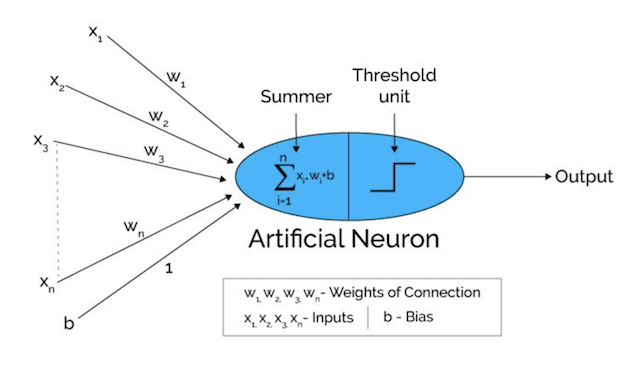
\includegraphics[width=0.7\textwidth]{images/perceptron.png}
        \caption{Un model de perceptron\cite{adi-from-perceptron}}
    \end{center}
\end{figure}
\label{perceptron}

Modul de învățare a unui perceptron este foarte simplu: Dacă greșește în a clasifica un element (obține \textit{output} 1 când valoarea elementului e 0, sau invers) creștem ponderile dacă activarea a fost prea mică comparativ cu pragul de activare, respectiv descreștem ponderile dacă pragul de activare a fost mai mic decât activarea.
Astfel perceptronul își adaptează ponderile dinamic, în funcție de datele de antrenament, trecând printr-un proces de învățare.

De-a lungul istoriei, au fost folosite mai multe tipuri de neuroni, fiecare având avantajele și dezavantajele sale. Cum corpul neuronului este în principiu un sumator ponderat, ce se va schimba între tipurile de neuroni este funcția de activare.

Deoarece de unul singur un neuron nu are putere de decizie prea mare, o rețea neurală va folosi mai mulți,  ieșirile unor neuroni constituind intrări pentru alți neuroni. Neuronii vor comunica între ei prin activarea/lipsa activării, astfel imitând transmiterea de semnale electrice din cadrul creierului uman. 

O rețea neurală cu mai multe straturi de neuroni mai este numită și \textit{MultiLayerPerceptron}, deși de obicei sunt folosiți neuroni de tip sigmoid, nu perceptron. O rețea de tip este organizată tipic pe mai multe straturi, având urmatoarea structură:

\begin{figure}[!htbp]
    \begin{center}
        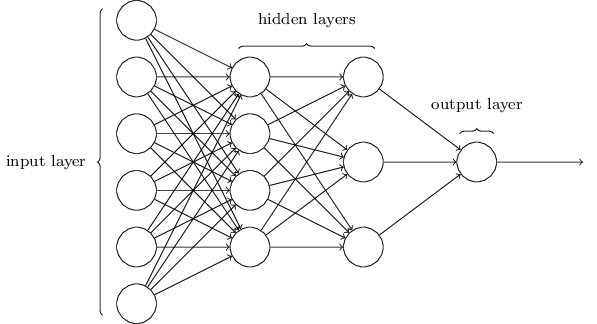
\includegraphics[width=0.9\textwidth]{images/retea.png}
        \caption{Structura unei rețele\cite{Nielsen2015}}
    \end{center}
\end{figure}

Straturile rețelei:
\begin{enumerate}
    \item Stratul de intrare (\textit{input})
    
    Stratul de \textit{input} este format din neuroni de intrare, care preiau datele de intrare și le transmit mai departe rețelei. De cele mai multe ori, neuronii de intrare nu au ponderi și nici funcții de activare, având un rol pasiv în cadrul rețelei.
    
    \item Stratul/Straturile de procesare (\textit{hidden})
    
    Straturile \textit{hidden} se ocupă de procesarea datelor de intrare. Există diferite moduri de a organiza straturile ascunse ale rețelei, în funcție de tipul rețelei: în cadrul unei rețele \textit{feedforward} doar vor transmite datele prelucrate,iar în cadrul unei rețele convoluționale ce se ocupă de procesarea imaginilor vor exista straturi convoluționale și de \textit{pooling} pentru a descoperi anumite trăsături în imagine, iar la rețelele de tip recurent, în straturile ascunse vor apărea conceptele de memorie și stări.
    
    În toate cazurile, ideea de bază este ca straturile \textit{hidden} vor prelua datele de intrare neprelucrate de la stratul de input, apoi vor prelucra acele date conform ponderilor asignate și calculate în diverse moduri, pasând apoi datele procesate ultimului strat, cel de ieșire. Numărul de straturi\textit{hidden}, organizarea lor, precum și tipurile de straturi și neuroni folosite depind atât de structura rețelei cât și de scopul în care este folosită aceasta.
    
    \item Stratul de ieșire (\textit{output})
    
    Neuronii din stratul de ieșire pot fi proiectați diferit  față de straturile anterioare, reprezentând actorii finali ai rețelei și având rolul de a produce outputul programului. Astfel, stratul de ieșire se coalizează și produce în mod concret rezultatul final, cu rol în eficientizarea și îmbunătățirea acestuia.
    Referitor la cele menționate anterior, pentru a înțelege mai bine rețeaua neurală, cele trei nivele de straturi(stratul de intrare, straturile ascunse și stratul de ieșire)vor fi privite împreună ca întreg.

\end{enumerate}

Pe lângă straturile descrise, o rețea neuronală mai are o funcție de cost folosită pentru a aproxima diferența dintre valoarea prezisă de rețea și valoarea reală. Mecanismul de antrenare utilizat la perceptron nu funcționează și aici, deoarece eroarea nu se propagă decât pe ultimul strat ascuns. Antrenarea unei rețele neurale are ca scop principal reducerea valorii funcției de cost, existând mai multe tehnici pentru a îmbunătați acest procedeu. Un rol foarte important în antrenarea unei rețele îl are algoritmul de \textit{Backpropagation}.

\textit{\textbf{Backpropagation}}
Când antrenăm un simplu perceptron, îi putem modifica instant ponderile în funcție de eroarea obținută (valoarea funcției de cost). În cazul unei rețele eroarea trebuie corectată la toate nivelele, nu doar la ultimul. Aici intervine algoritmul de \textit{Backpropagation}.
Algoritmul funcționează astfel:\cite{benchea-course}

Pentru fiecare strat \textit{l}, începând cu ultimul:

\quad Pentru fiecare neuron \textit{i} de pe stratul \textit{l}:
\begin{enumerate}
    \item Calculăm eroarea neuronului \textit{i} de pe stratul \textit{l}
    \item Folosind eroarea calculată calculăm derivatele parțiale ale funcției de cost în funcție de pragul neuronului \textit{i} și ponderile sale (derivatele parțiale ne arată cum variază funcția de cost în funcție de parametrii aleși)
    \item Modificăm ponderile și/sau pragul pentru a corecta eroarea pentru acel neuron
    \item Propagăm eroarea către neuronii de pe stratul \textit{l-1} și repetăm pașii de mai sus
\end{enumerate}{}

\begin{figure}[!htbp]
    \begin{center}
        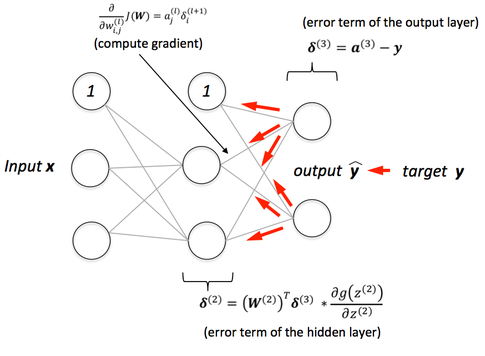
\includegraphics[width=0.8\textwidth]{images/backpropagation.png}
        \caption{Algoritmul de Backpropagation\cite{backpropagation}}
    \end{center}
\end{figure}

Atât în timpul antrenării, cât și în timpul folosirii unei rețele (trecerea datelor de intrare prin rețea pentru a obține date de ieșire), se folosește foarte mult înmulțirea de matrici (pentru a înmulți ponderile neuronilor cu datele de intrare). Pentru anumite cazuri de input, putem optimiza numărul de parametri și procesul de funcționare. În continuare vom prezenta un tip de rețea optimizată în mod special pentru imagini.

\section{Rețele neurale convoluționale}
 O rețea neurală convoluțională este un tip specializat de rețea neurală pentru procesarea datelor organizate sub o formă de tablou (un tablou unidimensional pentru datele temporale, un tablou bidimensional de pixeli pentru imagini) care folosește o operație matematică specializată numită convoluție în locul înmulțirii generale de matrici.\cite{Goodfellow-et-al-2016}
 
 O rețea convoluțională are anumite tipuri de straturi care nu apar într-o rețea clasică: straturi convoluționale și straturi de \textit{pooling}, dar la final apar și straturi conectate(\textit{fully-connected}) similare cu cele clasice.  În cadrul straturilor convoluționale și celor de \textit{pooling} neuronii din fiecare strat vor fi conectați doar la o mică regiune din stratul precedent, în loc de conexiuni între toți neuronii cum aveam la o arhitectură clasică.
 
 \begin{figure}[!htbp]
    \begin{center}
        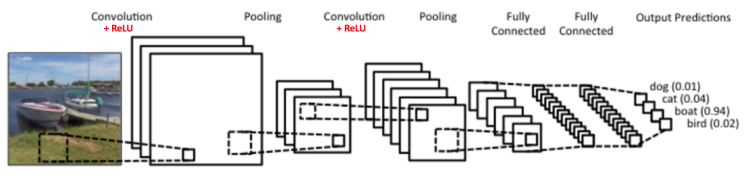
\includegraphics[width=0.8\textwidth]{images/convolutional_network.png}
        \caption{Arhitectura unei rețele convoluționale\cite{intuitive-explanation-conv}}
    \end{center}
\end{figure}

\subsection{Convoluția}
 În cadrul unui strat de convoluție se folosește un filtru( sau \textit{kernel}) pentru a extrage trăsături din cadrul imaginii. Filtrul se aplică unei mici regiuni din stratul precedent, realizând o mapare a imaginii în funcție de acel filtru. Cum imaginea este un tablou bidimensional de pixeli, un filtru va fi reprezentat tot de către un tablou bidimensional, mai mic decât cel de intrare. Aplicarea filtrului presupune calcularea produsului scalar între o parte din imagine de mărimea filtrului și filtru, efectuând această operație pentru toate părțile de aceeași mărime din imagine, luate la rând.
 
 Un exemplu de aplicare a unui filtru pe o imagine:
 
 \begin{figure}[!htbp]
    \begin{center}
        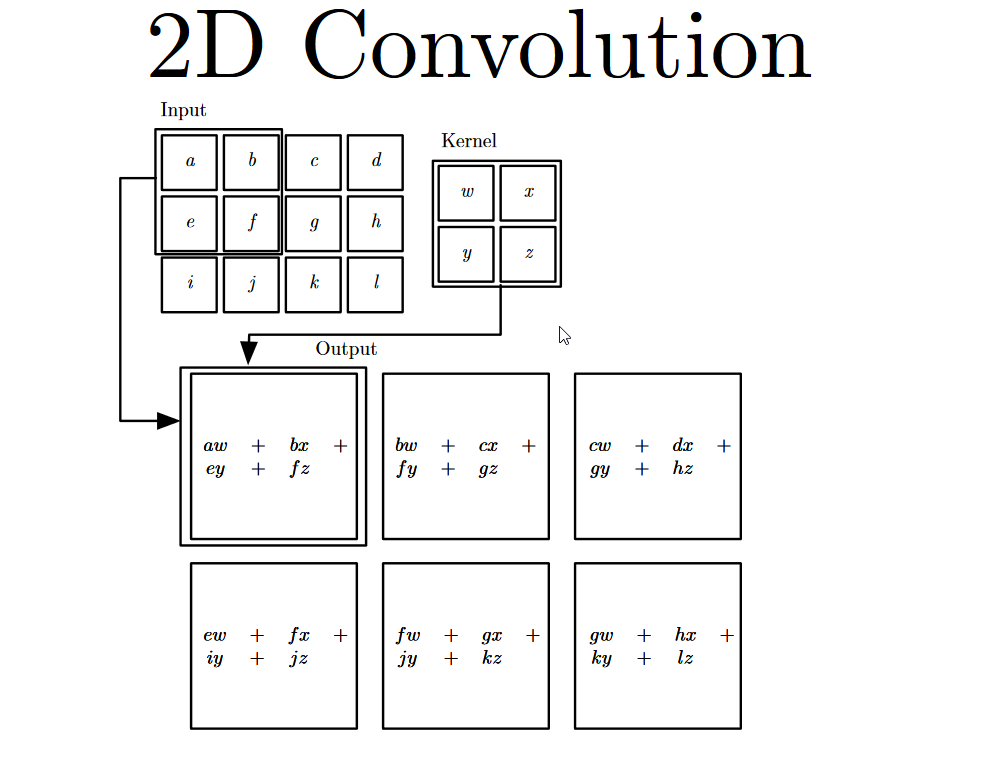
\includegraphics[width=0.9\textwidth]{images/filtru.png}
        \caption{Operația de convoluție \cite{Goodfellow-et-al-2016}}
    \end{center}
\end{figure}


\subsection{\textit{Pooling}}
Straturile de \textit{pooling} (denumite și straturi de \textit{subsampling} sau \textit{downsampling}) vor prelua câte o mapare a imaginii dată de un filtru convoluțional și vor reduce dimensiunea fiecărei mapări, extrăgând astfel trăsăturile dominante. Pot exista mai multe tipuri de straturi de \textit{pooling}: \textit{MaxPooling}, \textit{AveragePooling}, etc. De exemplu, în cazul operației de \textit{MaxPooling} ne alegem o zonă din mapare, din care extragem doar elementul maxim, astfel reducând dimensiunea mapării.

\begin{figure}[!htbp]
    \begin{center}
        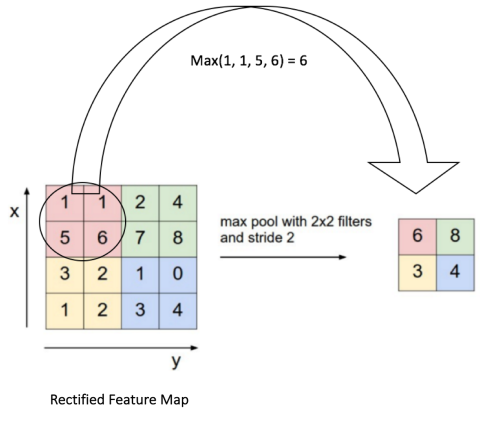
\includegraphics[width=0.7\textwidth]{images/pooling.png}
        \caption{Exemplu de \textit{MaxPooling}\cite{intuitive-explanation-conv}}
    \end{center}
\end{figure}

\subsection{\textit{Clasificare}}
 Adăugarea unui strat \textit{fully-connected} ajută la clasificarea imaginii.Stratul de clasificare este de fapt un \textit{MLP} tradițional, cu toți neuronii din el având conexiuni cu toți neuronii din stratul precedent. Stratul de clasificare va prelua trăsăturile de nivel înalt din imagine furnizate de straturile convoluționale și reduse ca dimensiune de straturile de pooling și va realiza o clasificare a imaginii bazată pe trăsăturile întâlnite.

Există multe tipuri de arhitecturi de rețele convoluționale, însă mai toate își au bazele pe operațiile descrise: convoluție, scalarea mapării(\textit{pooling}), apoi clasificare.


\section{Keras și Tensorflow}
\subsection{Tensorflow}
Tensorflow este un \textit{framework} cu sursă deschisă  dezvoltat de Google și folosit pentru calcule numerice. Tensorflow oferă suport pentru învățare automată și \textit{deep learning}. Folosind diverse instrumente puse la dispoziție, utilizatorii pot construi modele de învățare automată la nivele diferite de abstractizare, de la modele construite pe baza unor serii de operații matematice la API-uri de nivel înalt pentru construirea de arhitecturi întregi prerealizate, cum ar fi rețele neurale sau regresori liniari.

\subsection{Keras}
Keras reprezintă un API de nivel foarte înalt dedicat rețelelor neurale, scris în Python și care poate rula pe mai multe platforme de învățare automată cum ar fi TensorFlow, CNTK sau Theano. A fost dezvoltat pentru a abstractiza la maximum procesul de creare a unei rețele neurale, având ca scop atât experimentarea rapidă, cât și construcția într-un mod facil a unei arhitecturi solide. Keras poate fi văzut ca o interfață simplă, consistentă, folosită pentru cazurile uzuale, ce se pliază peste un \textit{back-end} optimizat de \textit{deep learning} și învățare automată. Este extrem de modular, permițând reutilizarea de blocuri configurabile, dar și extensibil, utilizatorii având posibilitatea de a crea noi straturi, funcții de cost sau arhitecturi pentru idei de cercetare. 

